\documentclass[9pt]{beamer}
\usetheme{Boadilla}
\usepackage[utf8]{inputenc}
\usepackage{amsmath}
\usepackage{amsfonts}
\usepackage{amssymb}
\usepackage{graphicx}
\usepackage{subfig}
\usepackage[export]{adjustbox}
\usepackage{xcolor}

\setbeamercolor{block title}{fg=white, bg = cyan }

\newcommand{\disappear}[1]{} %hide slides


\author[Adriano, Germano, Simone]{Adriano Del Vincio, Germano Bonomi,\\ Simone Stracka}
\title[Alpha 2]{Studying Annihilation Distributions \hrule}
%\setbeamercovered{transparent} 
%\setbeamertemplate{navigation symbols}{} 
\logo{
\includegraphics[width = 0.125\textwidth]{../logo/ALPHA_Logo.jpg}}
\newcommand{\nologo}{\setbeamertemplate{logo}{}}
\institute[]{University of Brescia, INFN Pisa} 
\titlegraphic{
\begin{figure}
\hspace{1.cm}

\includegraphics[width = 0.12\textwidth ]{../logo/logounibs.png}
%\hspace{1cm}

\includegraphics[width = 0.25\textwidth ]{../logo/1_Pisa_LOGO_SIGLA.pdf}
\end{figure}
}
\date{13/11/2023} 
\subject{ALPHA 2 spectroscopy, identifying the distinct contribution of $\overline{H}$ annihilation on the walls and the annihilation resulting from the residual gas.} 
%\setlength{\textfloatsep}{6 pt plus 1.0pt minus 2.0pt}
\begin{document}

\begin{frame}
\titlepage
\end{frame}

%\begin{frame}
%\tableofcontents
%\end{frame}

\disappear{
\begin{frame}{}

\begin{block}{Objective}
A procedure to disantangle the contribution of annihilations of antihydrogen on the trap walls and on the residual gas has been developed and tested.
It is based on a Maximum Likelihood fit of the radial distribution of the annihilations that has been tuned using an “ad-hoc” Monte Carlo simulation toy.
\end{block}

\begin{itemize}
\item The model/template for annihilations on the trap walls has been extracted from the 2-second mixing window.
\item The model/template for annihilations of the residual gas has been obtained using the losses when antihydrogen is hold in the trap (microwaves - UW - losses).
\item A model/template for the cosmic background is also used.
\end{itemize}

%The fitting procedure proved to be \textbf{stable and reliable} with the simulation toy. %and it has been tested also on a couple of runs.

The PDFs used for the fit procedure and the data generation the data are listed below:
\begin{itemize}
\item PDF Mixing: the Normal distribution
\item PDF Residual gas: Rayleigh distribution $\frac{r}{\sigma^{2}} e^{-\frac{r^{2}}{2 \sigma^{2}}}$
\item PDF Cosmic: $k \cdot x$
\end{itemize}

The factor $k$ is the normalization constant. The Mixing, residual gas and cosmic data \\ are fitted and the result are shown in the following slides.
\end{frame}
}

\begin{frame}{MIXING}

Mixing dataset represents almost pure data of anti-hydrogen annihilation on the walls. The radius distribution is fitted with a Gaussian.

\begin{figure}
\vspace{-2pt}
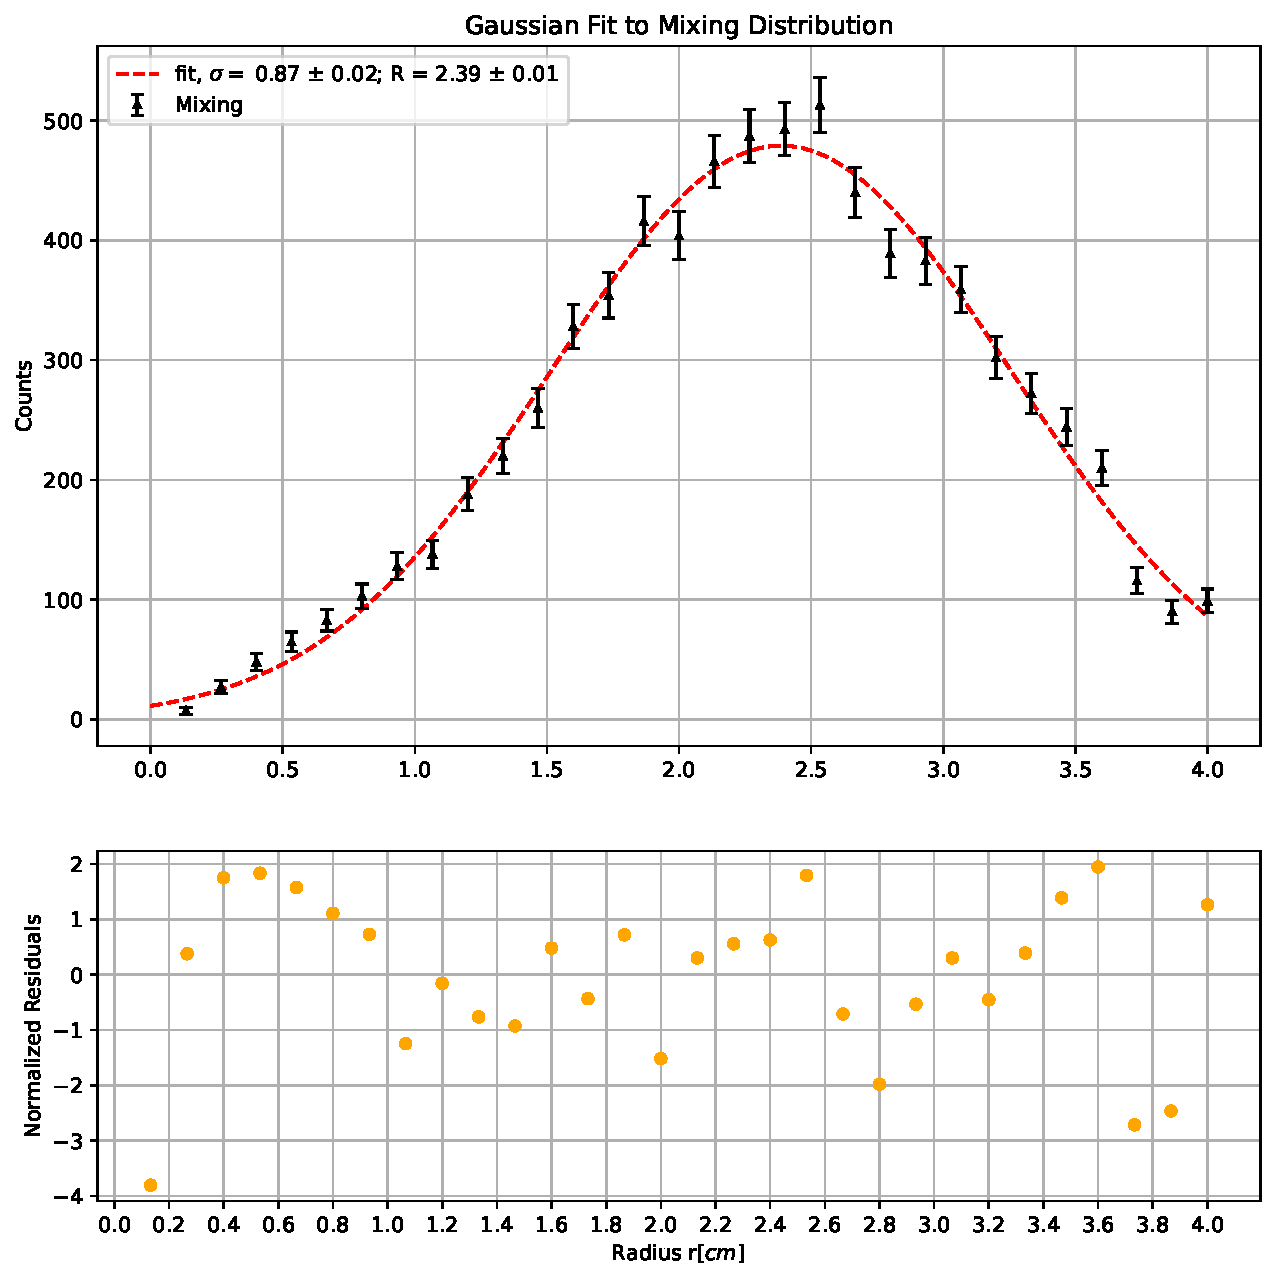
\includegraphics[width = 0.6\textwidth]{./SingleModel/GaussianFitMixing.pdf}
\end{figure}

\end{frame}

\begin{frame}{Residual Gas}

The microwave losses represent an almost pure anti-hydrogen sample of annihilation events due to residual gas inside the trap. The data are fitted with Rayleigh distribution $\frac{r}{\sigma^{2}} e^{-\frac{r^{2}}{2 \sigma^{2}}}$

\begin{figure}
\includegraphics[width = 0.60\textwidth]{./SingleModel/FitToUW.pdf}
\end{figure}

\end{frame}

\begin{frame}{Cosmic}

The cosmic distribution is obtained from a dataset without particles in the trap. A liner model $m \cdot x$ is assumed.

\begin{figure}
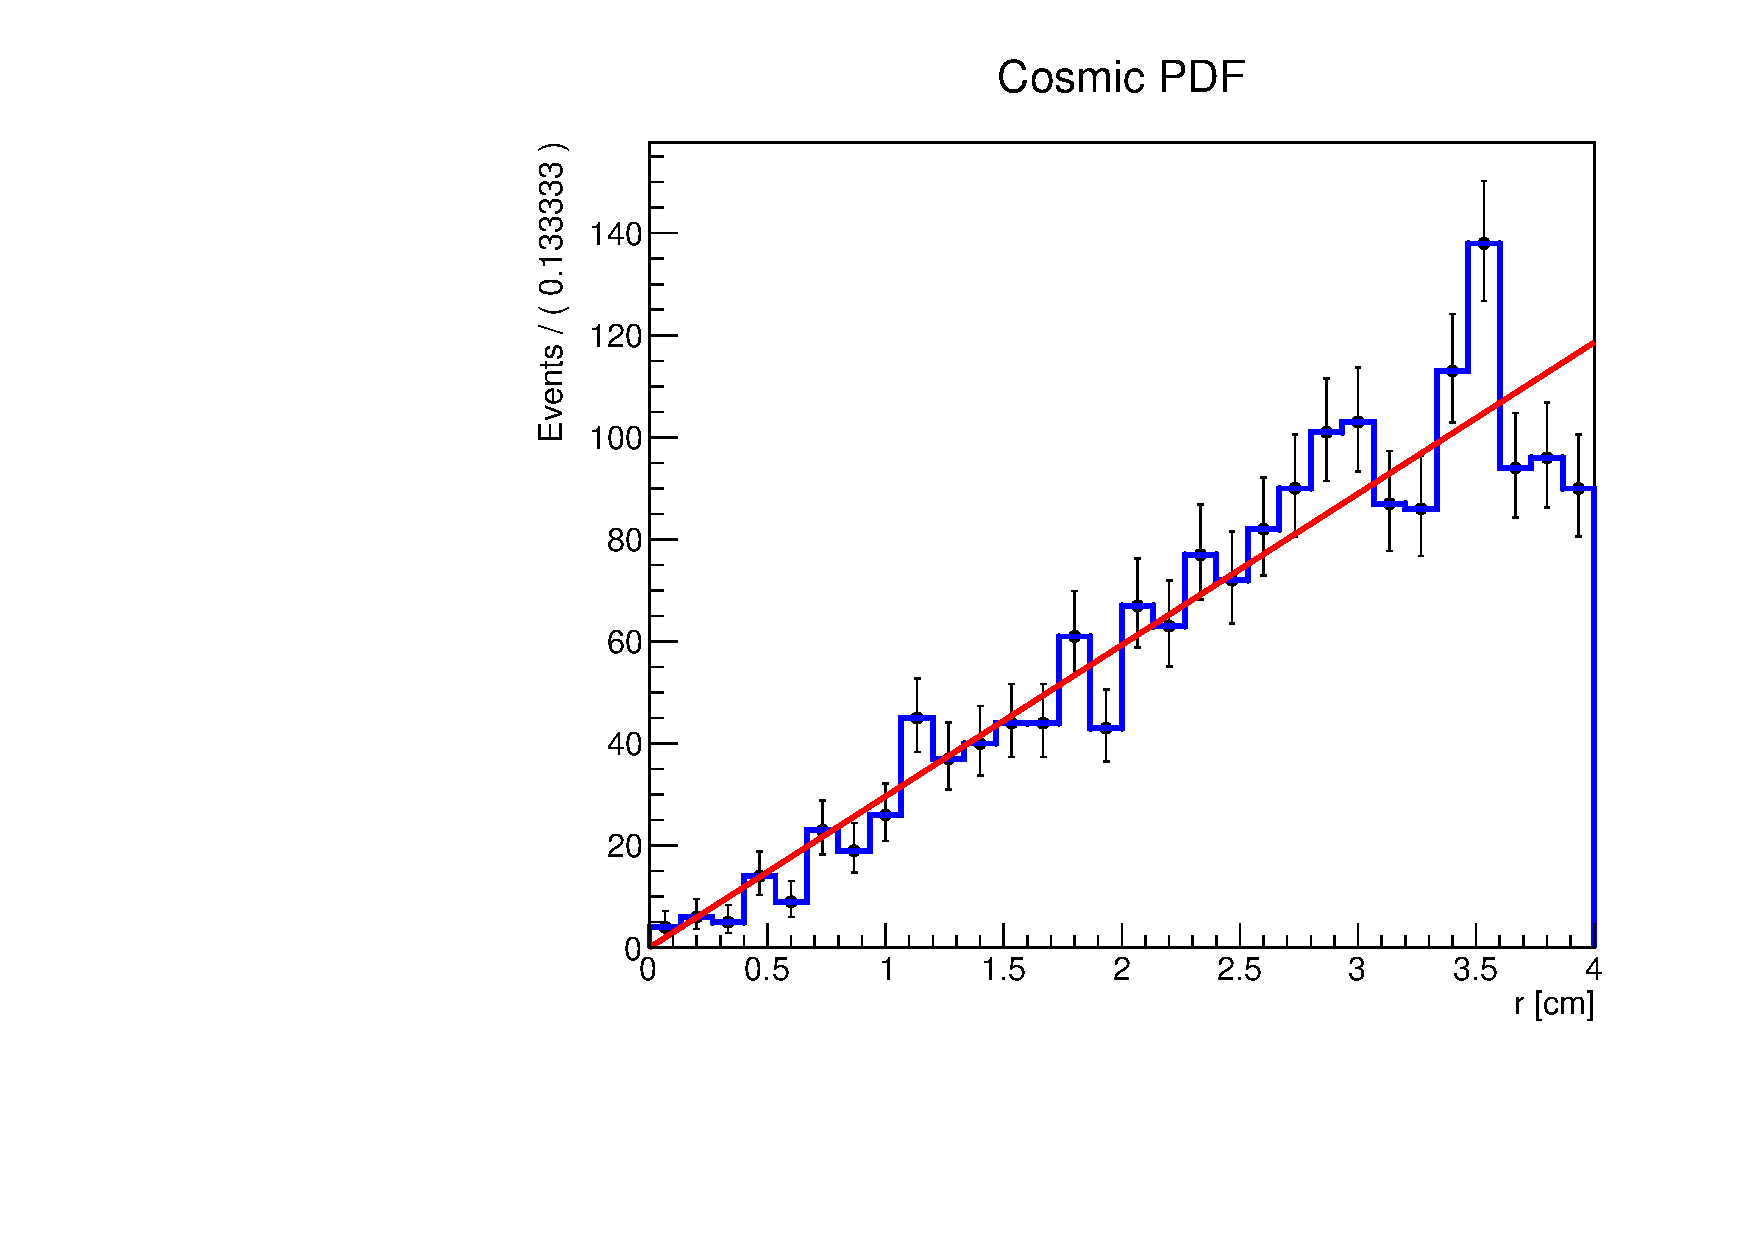
\includegraphics[width = 0.65\textwidth]{./SingleModel/Cosmici_fit.pdf}
\end{figure}

\end{frame}

\begin{frame}{PDFs normalized plotted together}
\begin{figure}
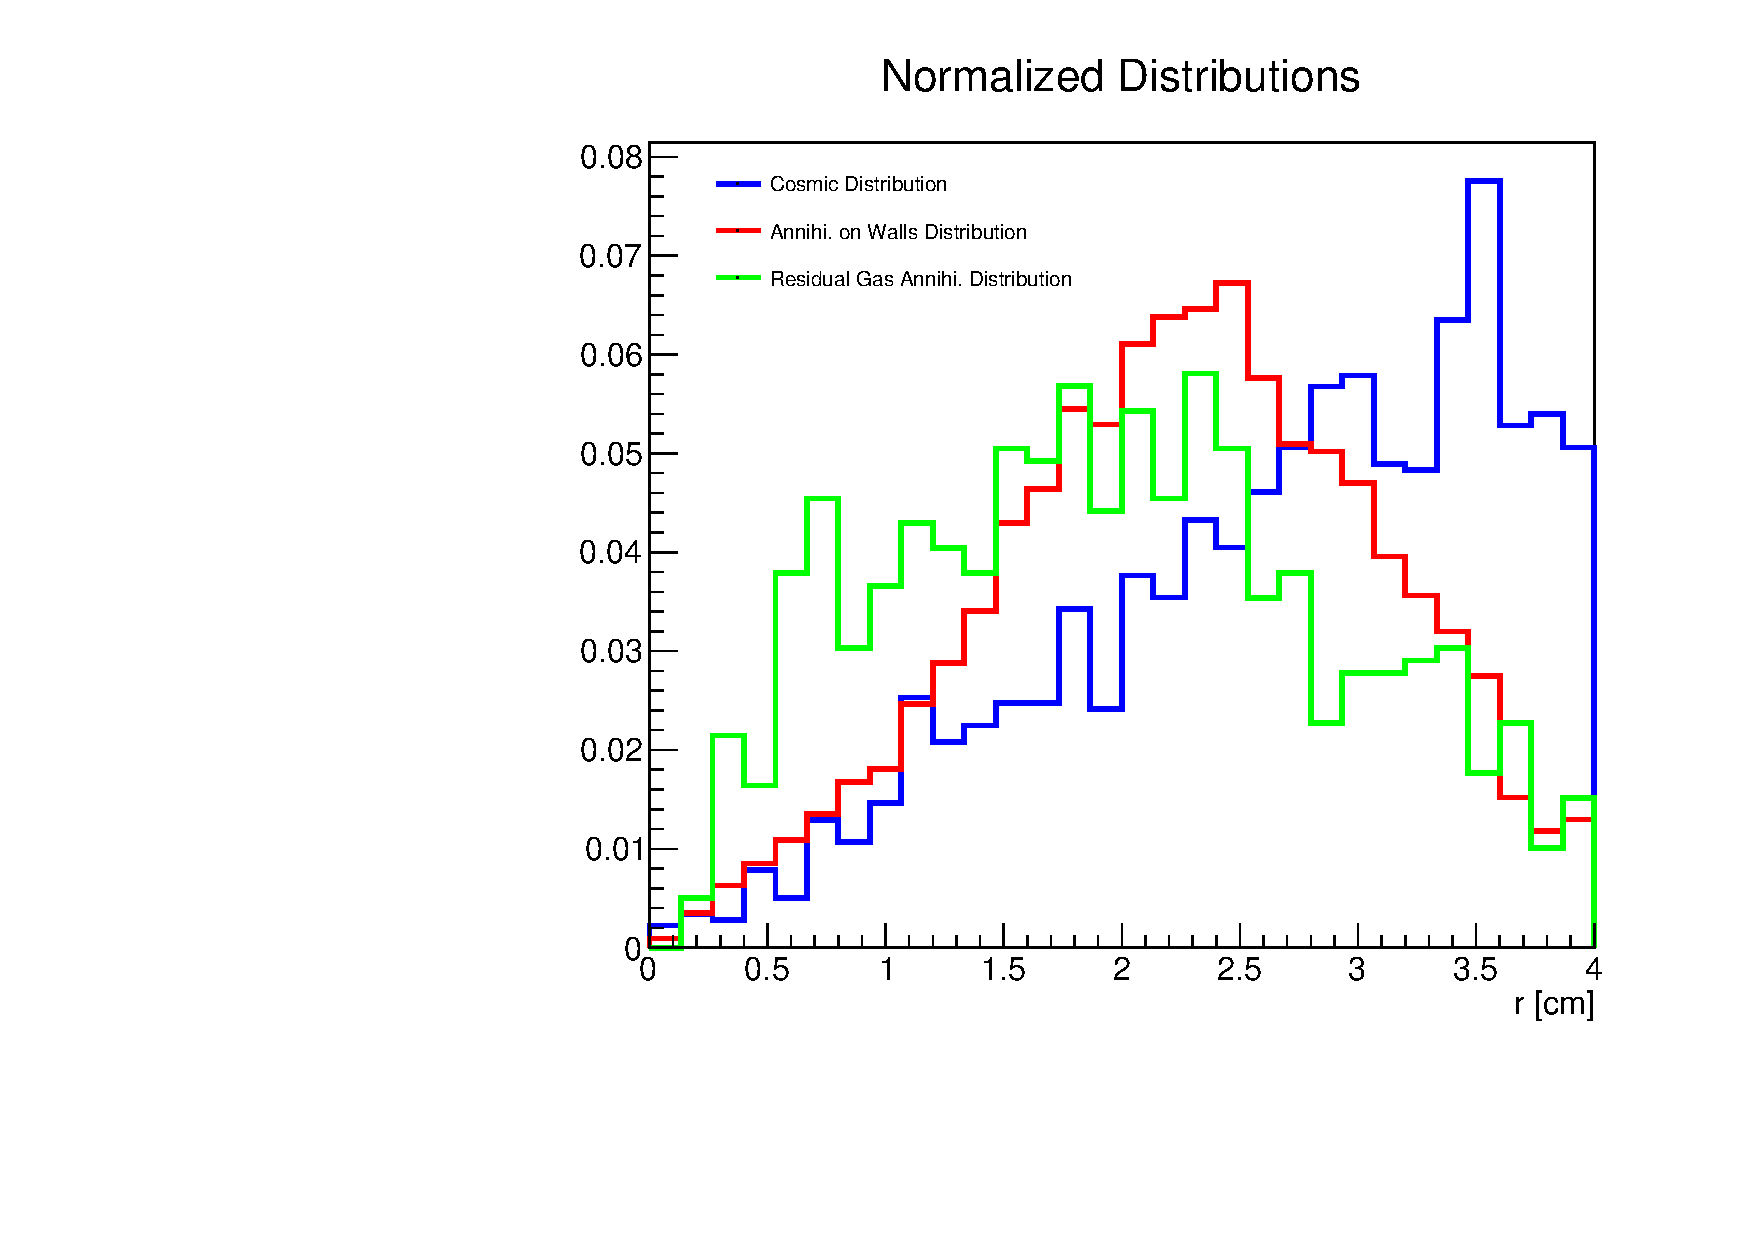
\includegraphics[width = 0.75\textwidth]{PdfTogether.pdf}
\end{figure}
\end{frame}

\begin{frame}{Radial Density}

The histogram in $r$ variable doesn't account for the different area of the bin which is $2 \pi r \cdot dr$. So it is useful to divide per $2 \pi r$ to obtain the radial density of the events.

\begin{figure}[hbtp]
\centering
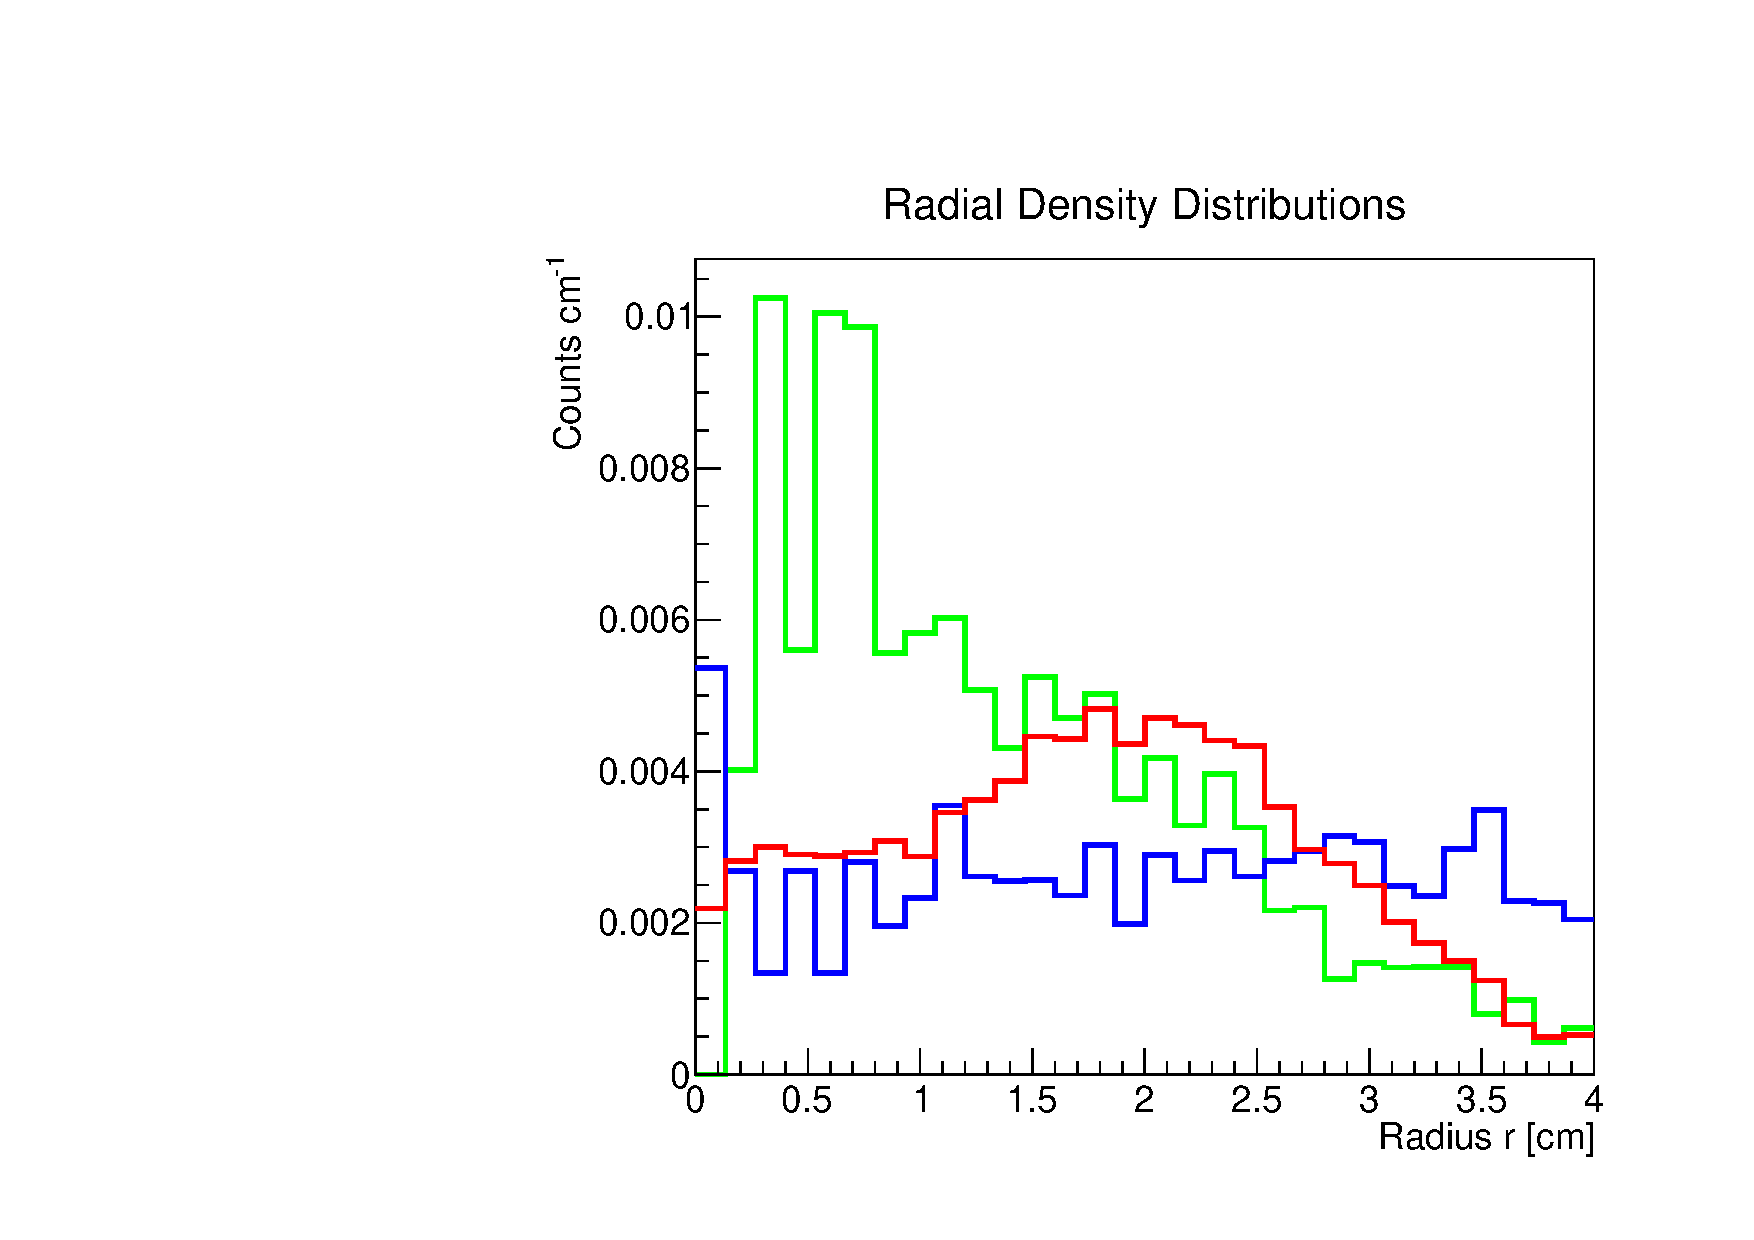
\includegraphics[width = 0.7\textwidth]{RadialDensity.pdf}
\disappear{\caption{Radial density for \texttt{r68465\_uw\_exp\_freq4.vertex} dataset}}
\end{figure}
\end{frame}

\begin{frame}[t]{Monte Carlo Simulation Toy}

To study the accuracy of the algorithm to reconstruct the various parameter, we have developed a "toy" simulation tool. The model to generate the data is:

\begin{equation}
F_{gen}(r) = N_{sample} \cdot (a \cdot PDF_{mix} + b \cdot PDF_{gas} + c \cdot PDF_{cosmic}) 
\end{equation}

where $a,b,c$ represent the "weights" of the various contributions to the PDF used to generate the data. The number of annihilation is indicated as $N_{sample}$. Once the data are generated, they are fitted with the model:

\begin{equation}
Nfit_{mix} \cdot PDF_{mix} + Nfit_{gas} \cdot PDF_{gas} + Nfit_{cosmic} \cdot PDF_{cosmic}
\end{equation}

The parameters of the fit are $Nfit_{mix}, Nfit_{gas}$ and $Nfit_{cosmic}$. The "true value" are defined as:

\begin{itemize}
\centering
\item $Ngen_{mix} = a \cdot N_{sample}$
\item $Ngen_{gas}  = b \cdot N_{sample}$
\item $Ngen_{cosmic}  = c \cdot N_{sample}$
\end{itemize} 

In generation $Ngen_{mix}$,$Ngen_{gas}$,$Ngen_{cosmic}$ are varied according to a Poissonian distribution. 
\end{frame}


\begin{frame}{Example of fit, Toy: $N_{sample} = 1000$, a = $33\%$, b = $33\%$, c = $33\%$}
\begin{center}
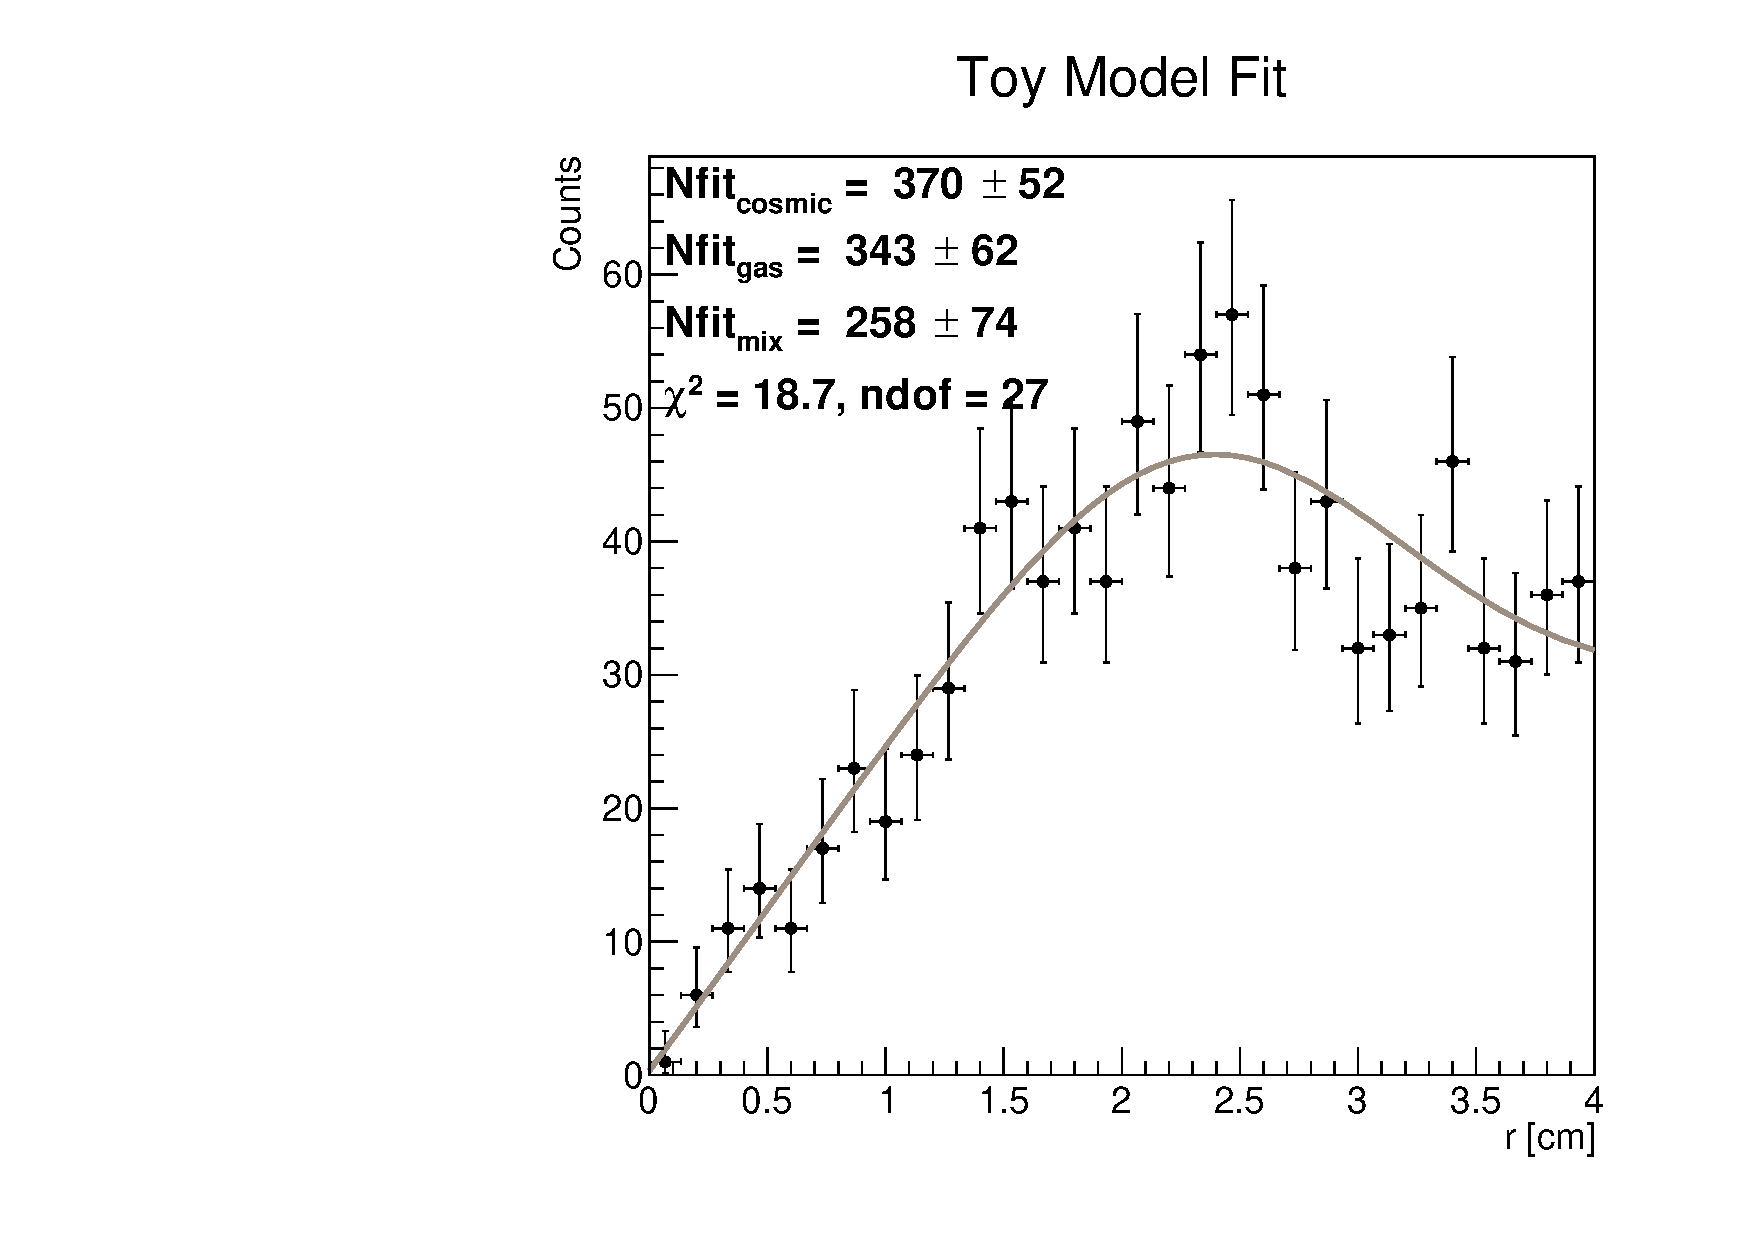
\includegraphics[width = 0.70\textwidth]{N1000/FitToy(33,33,33).pdf} 
\end{center}

\end{frame}

{\nologo
\begin{frame}[t]{Toy: $N_{sample} = 1000$, a = $ 33\%$, b = $33\%$, c = $33\%$}

In this plot we have fixed the weight of each distribution to $33\%$, with $N_{sample} = 1000$ and $N_{trials} = 1000$, to ensure that the algorithm is able to reconstruct the parameters, and check the presence of a bias.
The variable of the histograms are: $\dfrac{Nfit - Ngen}{\sigma_{fit}}$. The distributions are normal and the fit procedure is behaving as expected.

\begin{figure}[!t]
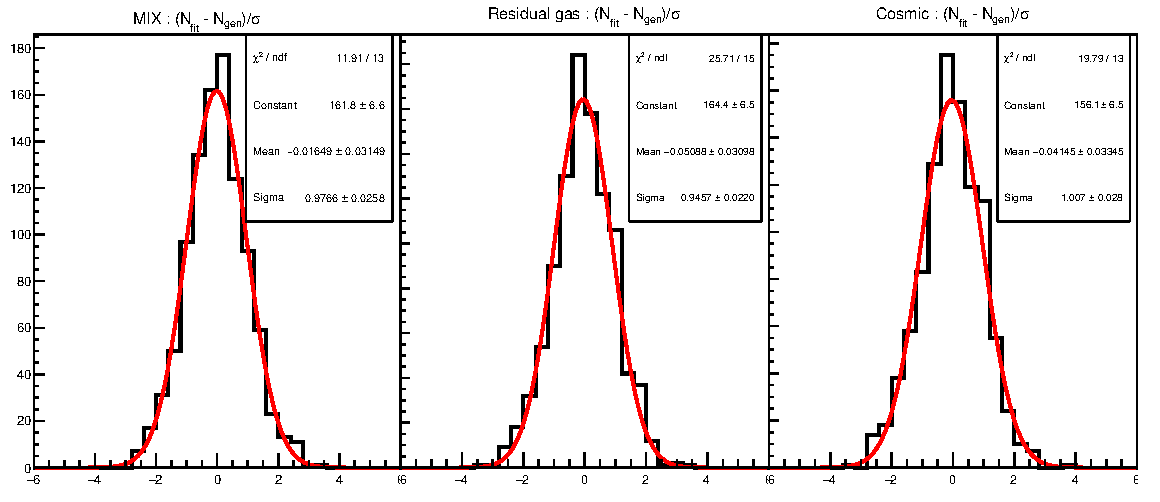
\includegraphics[width = 1\textwidth]{N1000/ToyNmix(33,33,33)-cropped.pdf} 
\end{figure}
\end{frame}
}
\disappear{
\begin{frame}{weight variation $a$ for mix.}

Now we study how the coefficients of the fit $Nfit_{mix}, Nfit_{uw}$ and $Nfit_{bk}$ vary with the increment of the weight $a$. 
At fixed $c = 10\%$, $a$ is raised from $0\%$ to $90\%$ and $b$ is decreased accordingly. 

\begin{figure}
\vspace{-7pt}
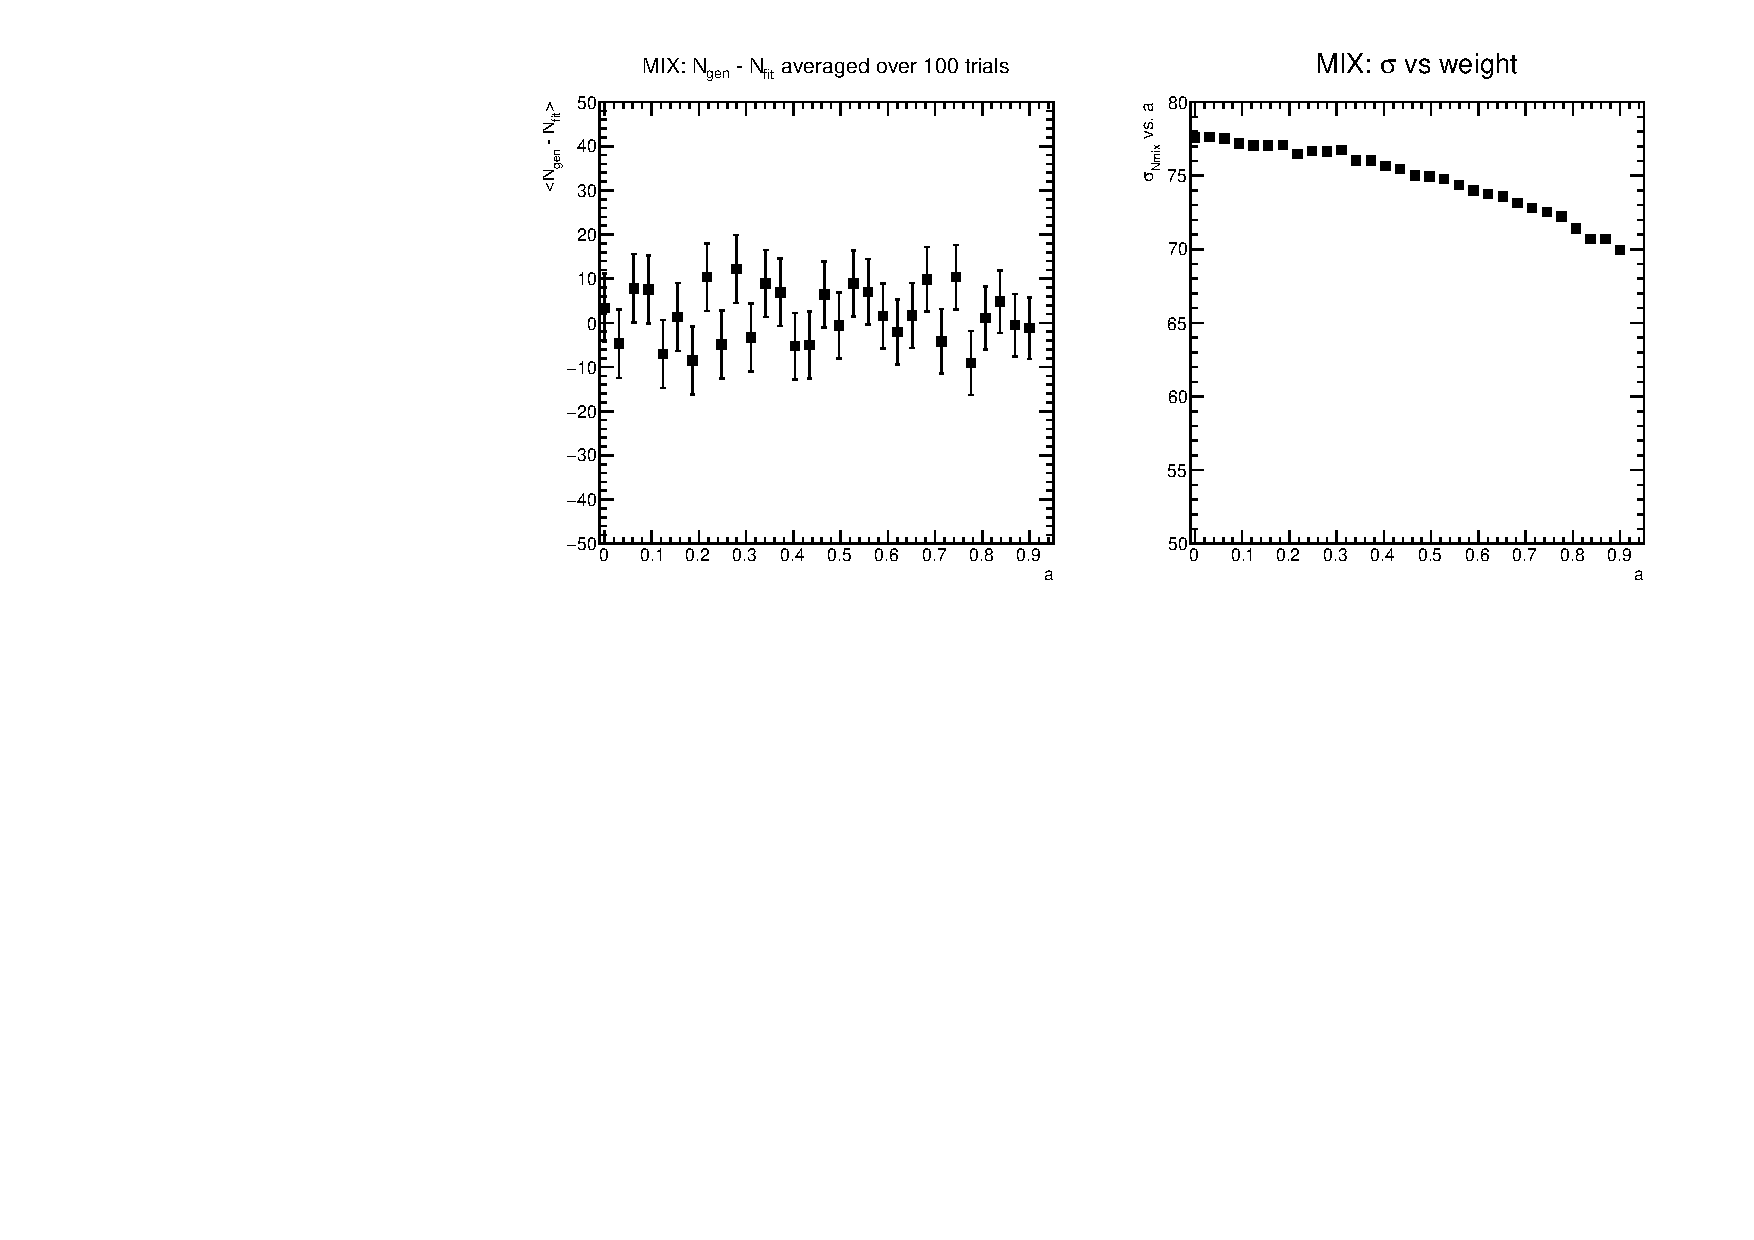
\includegraphics[width = 1\textwidth , valign = t]{N1000/Nmix_and_Sigma(90,0,10).pdf}
\end{figure}
The number events is always $ N_{sample} = 1000$. For each value of the weight $a$  we\\ iterate 100 times ($N_{trials} = 100$) to study the reconstructed coefficients with the \\ variation of the weights.
\end{frame}
}
{\nologo
\begin{frame}{$N_{sample} = 165$, $N_{trials} = 100$}
Now we study how the coefficients of the fit $Nfit_{mix}, Nfit_{gas}$ and $Nfit_{cosmic}$ vary with the increase of the weight $a$. $Nsample$ is fixed at $165$, to reproduce a typical amount of events in real data (such as for a frequency of run 68465, after applying \textit{cut1}). The value of $c$ is fixed to reproduce the number of expected events from background ($c = 6\%$, $Ngen_{cosmic} \simeq 10$).
\begin{figure}
\subfloat{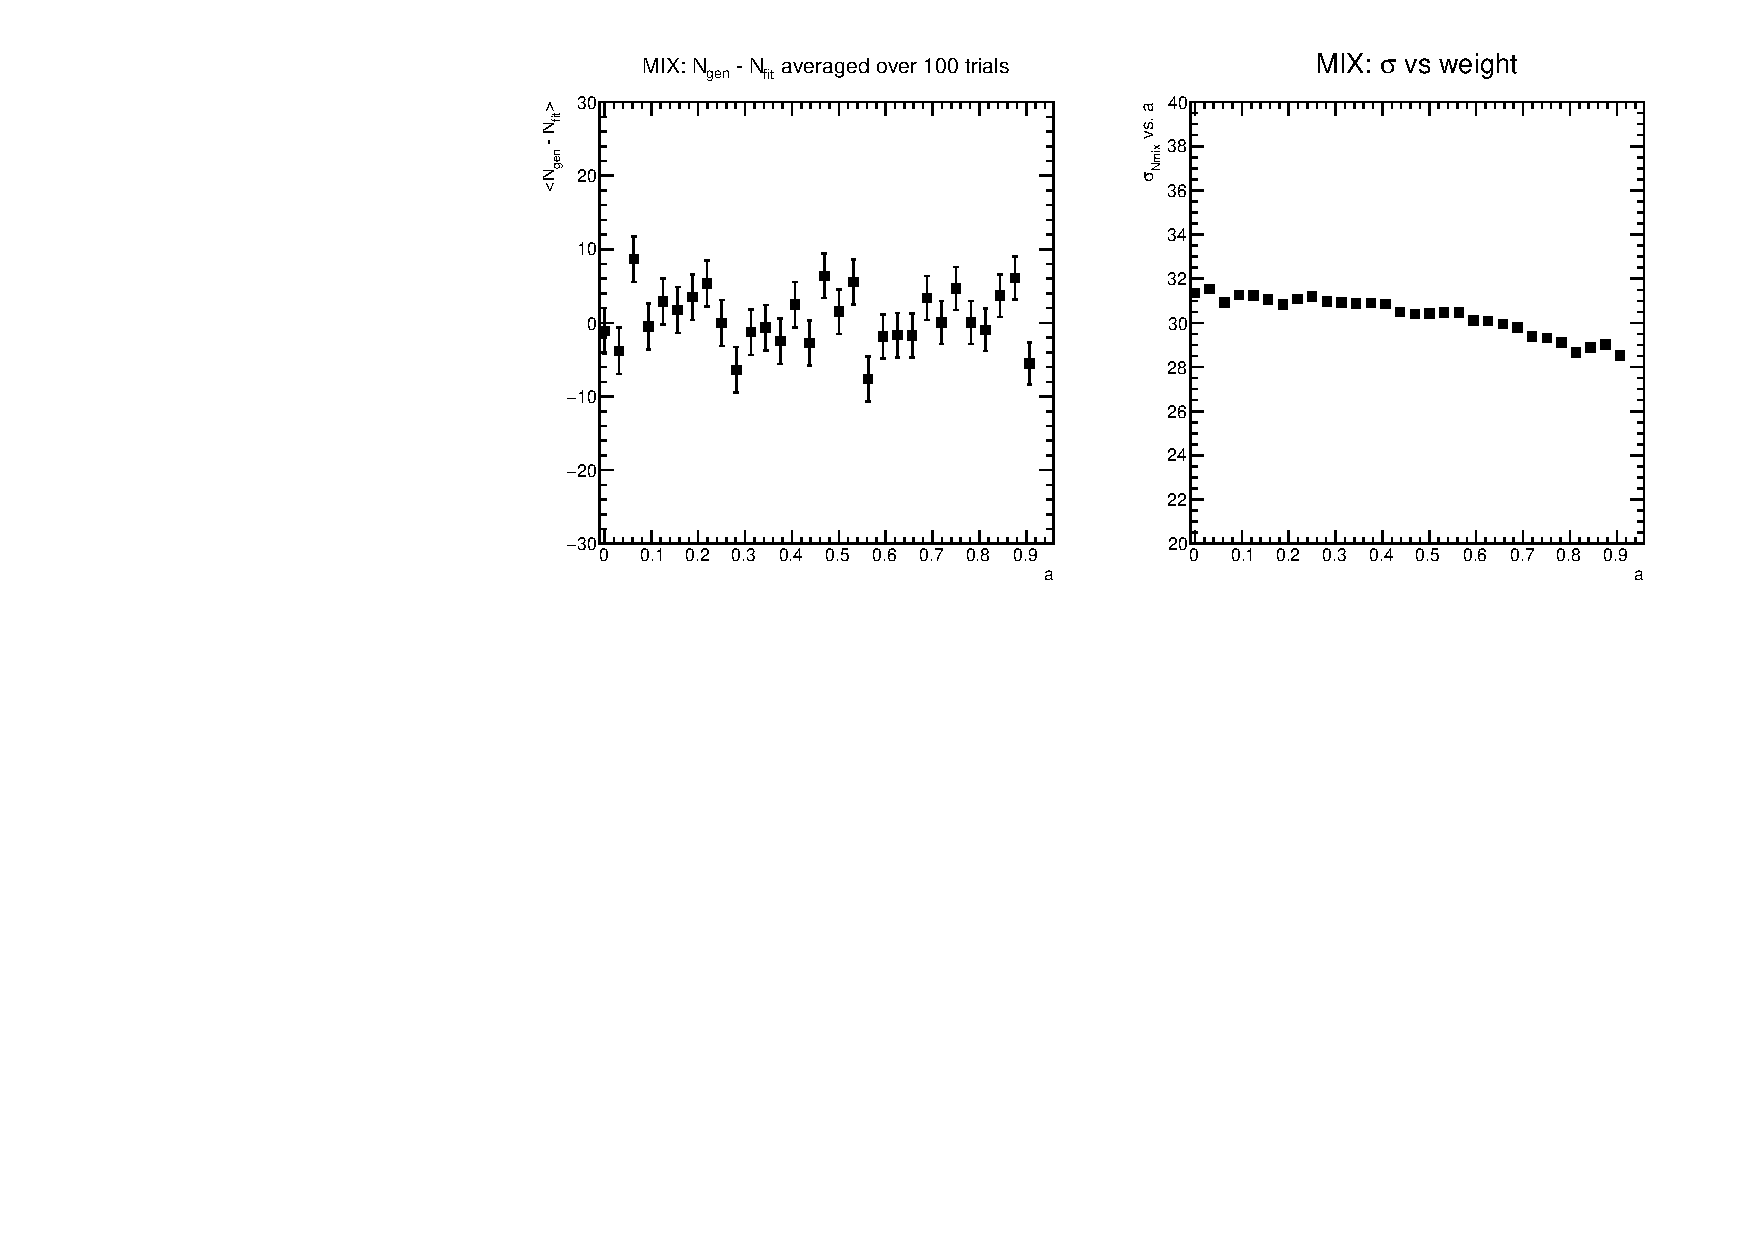
\includegraphics[width = 1\textwidth]{N165/Nmix_and_Sigma_bkFixed(93,0,6).pdf}}
\end{figure}
\end{frame}
}
\disappear{
\begin{frame}{Fitting the data, Test 1}

PDF = Gaussian (Mixing) + Rayleigh (Residual gas) + linear model (cosmic fixed).

Data taken from: run r68465

\begin{figure}[hbtp]
\centering
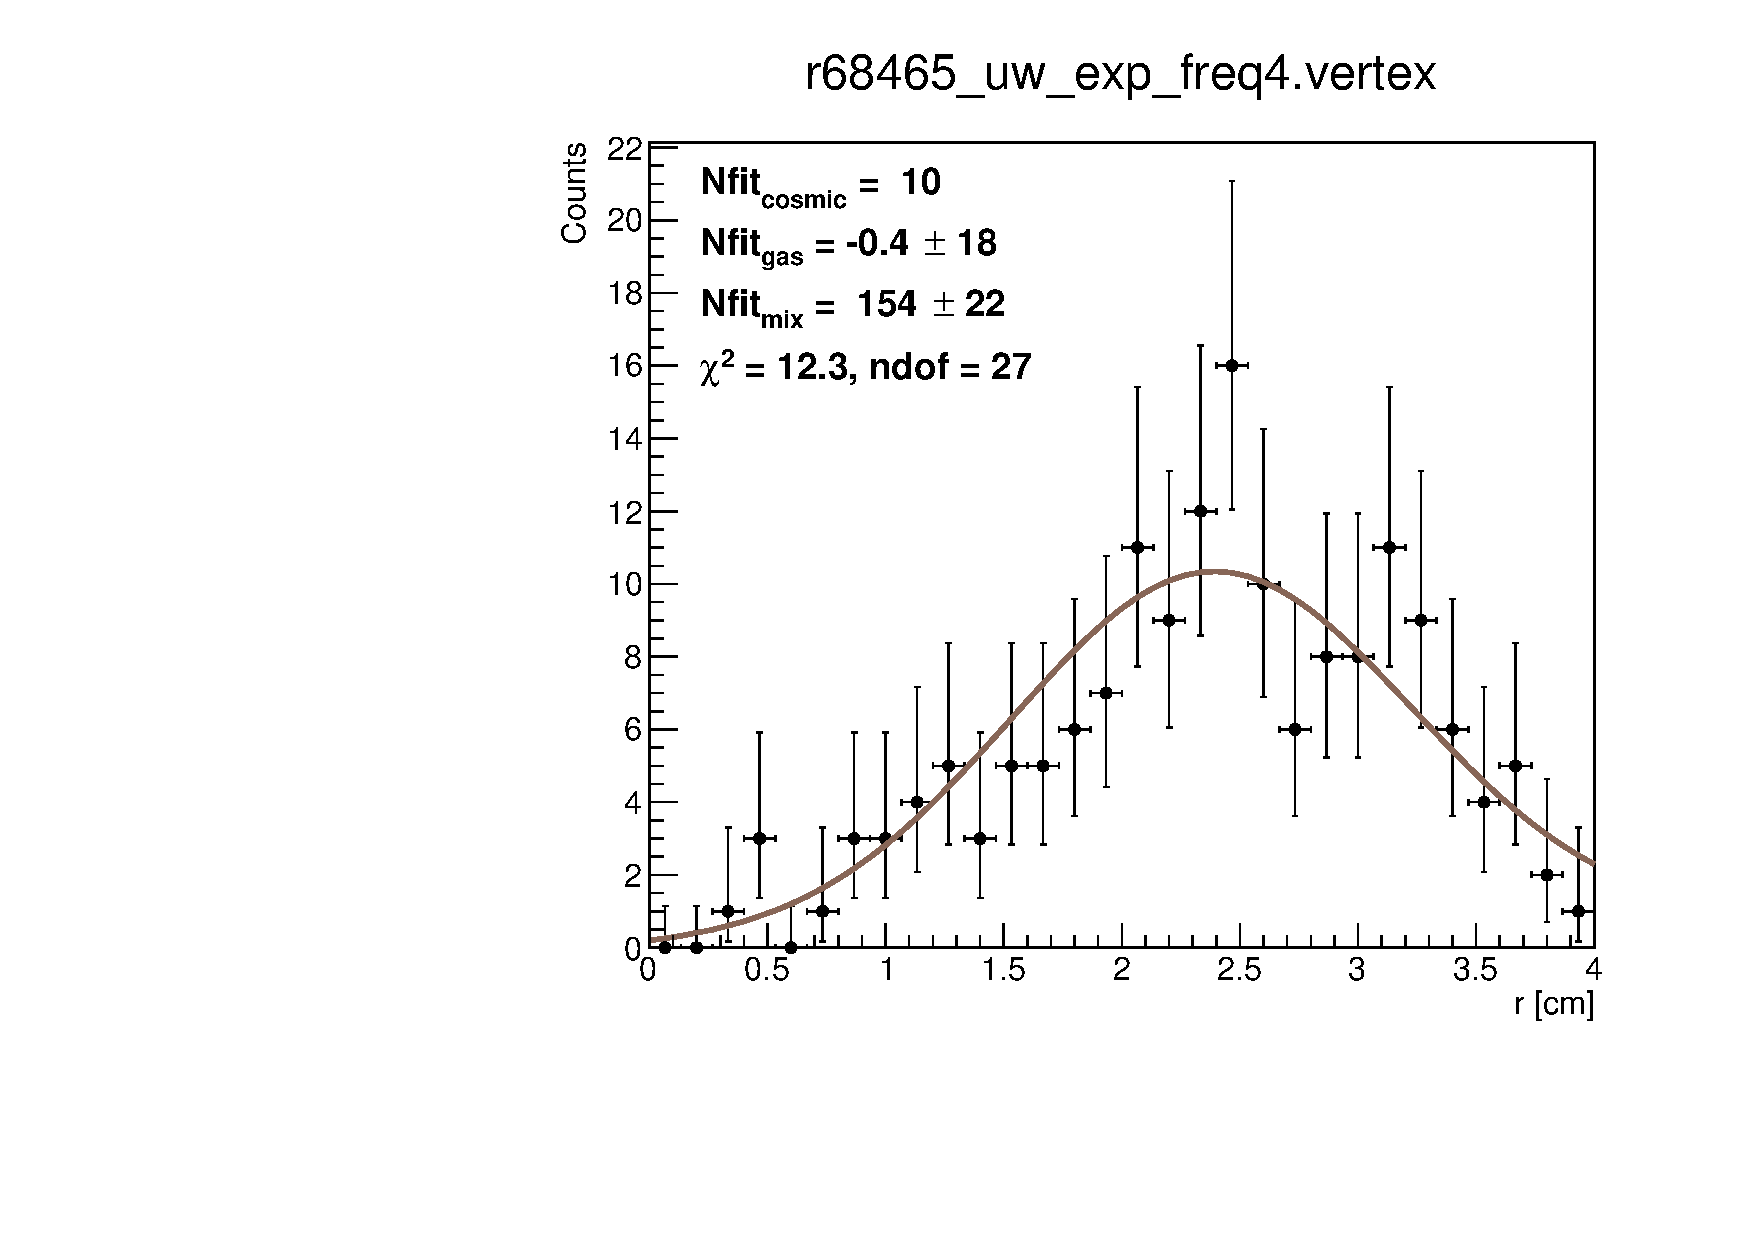
\includegraphics[width = 0.65 \textwidth]{./SingleModel/TuttoAnalitico.pdf}
\end{figure}
\end{frame}

\begin{frame}{Fitting the data, Test 2}

PDF = Gaussian (Mixing) + Rayleigh (Residual gas) + linear model (cosmic fixed).

Data taken from: \texttt{r68465\_uw\_exp\_freq5.vertex.csv}
\begin{figure}
\centering
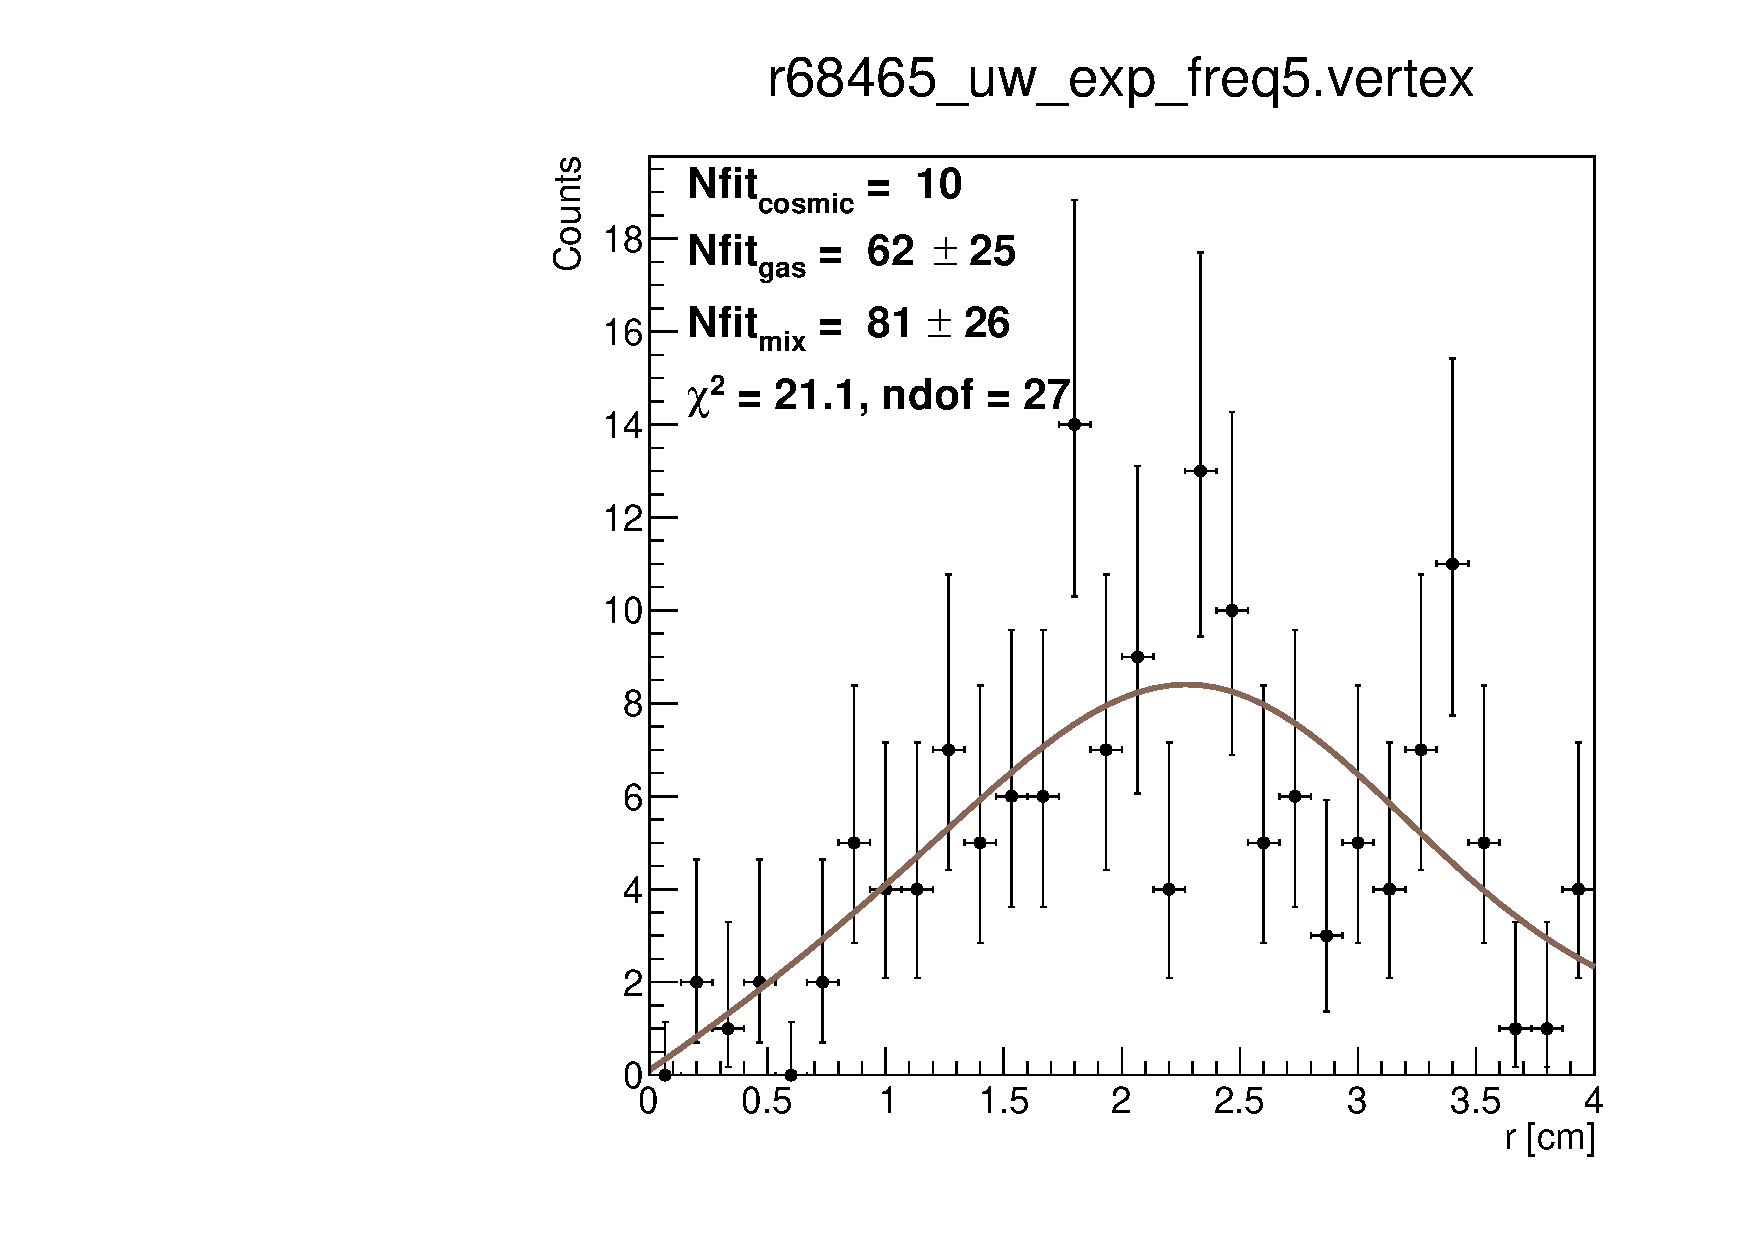
\includegraphics[width = 0.65 \textwidth]{./SingleModel/AnalyFit_2.pdf}
\end{figure}
\end{frame}
}

\disappear{
\begin{frame}[noframenumbering]
\begin{center}
\color{red}{\Large \bf{ADDITIONAL MATERIAL}}
\end{center}
\end{frame}

{\nologo
\begin{frame}{$N_{mix} - N_{fit}$ for $a = 46\%$, $b = 46\%$, $c = 6\%$.}
\begin{figure}
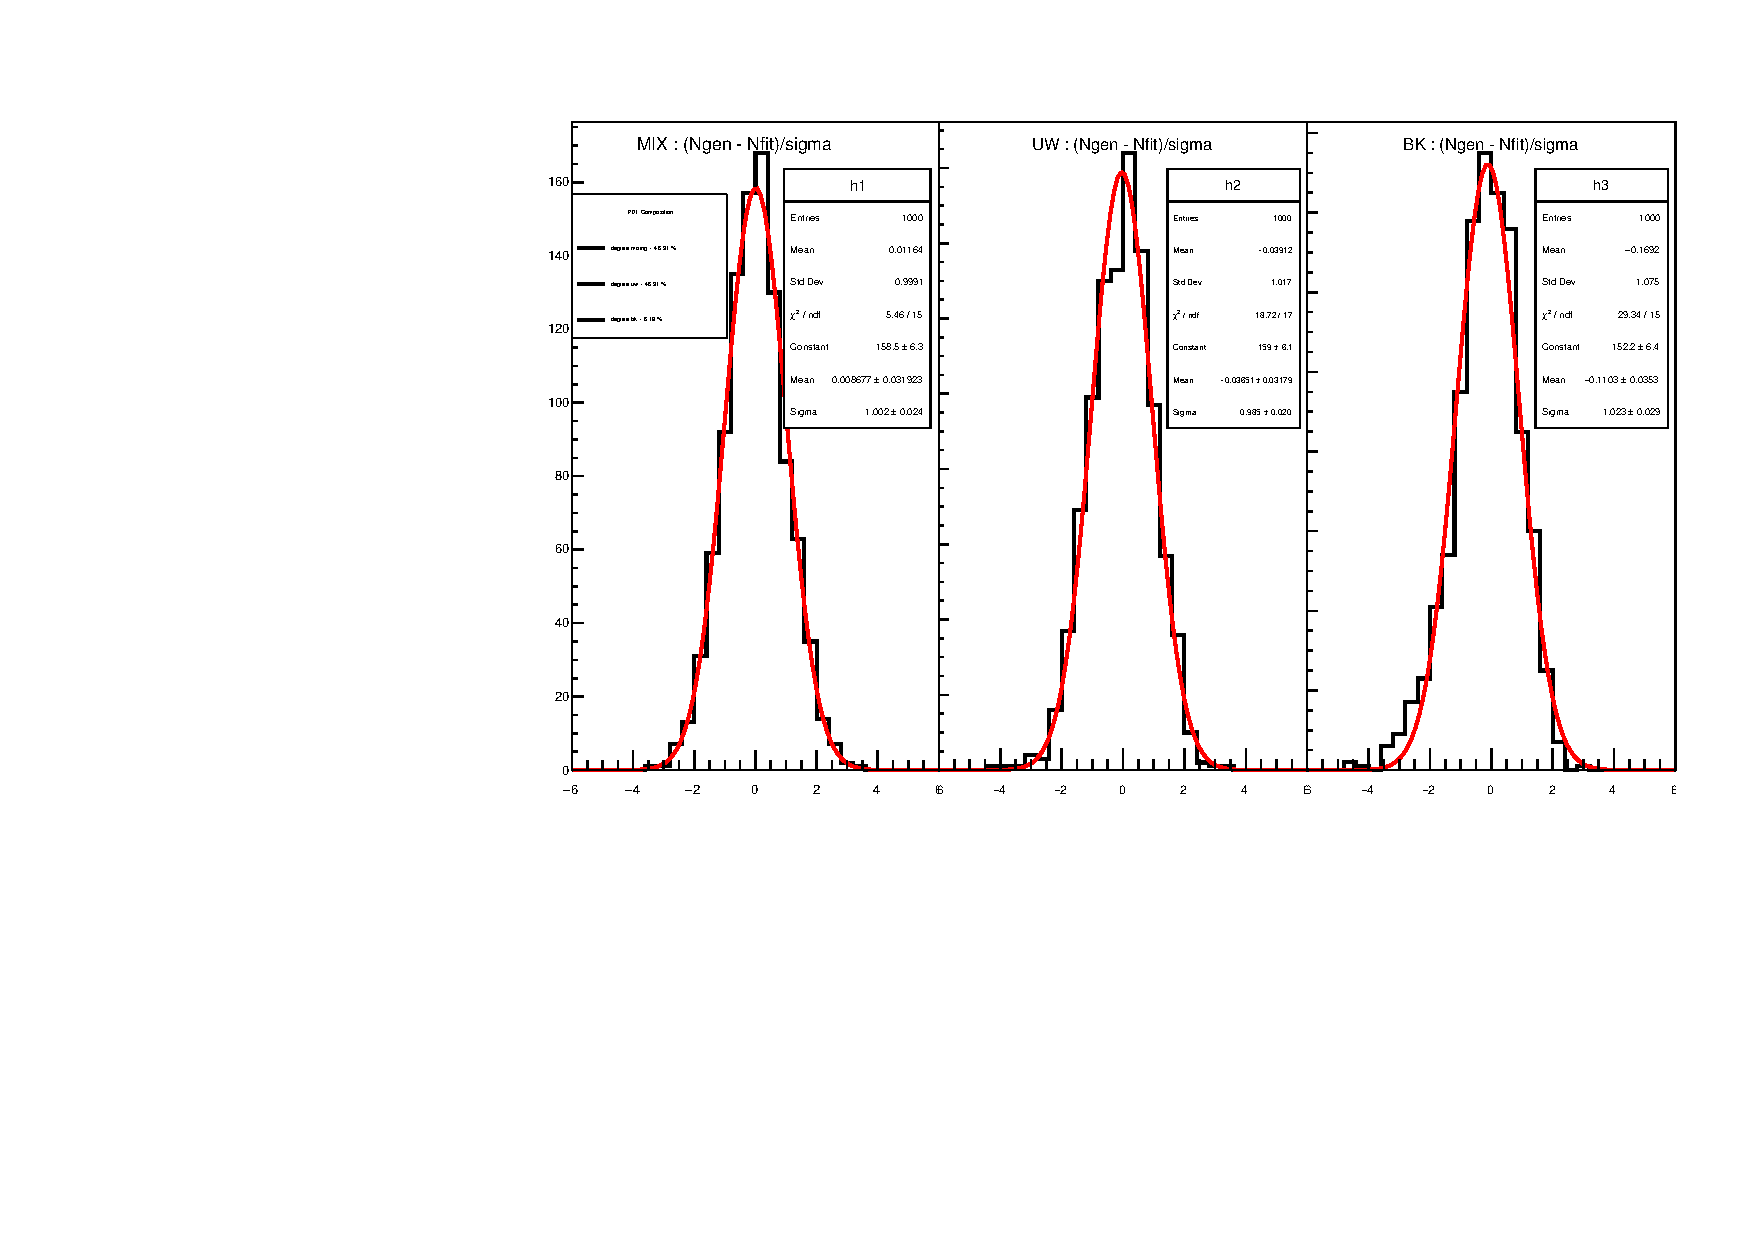
\includegraphics[width = 1\textwidth]{N165/ToyNmix(46,46,6).pdf}
\end{figure}
\end{frame}
}

{
\begin{frame}{$N_{uw}$ parameter of the fit model fixed}
The Toy simulation is tested fixing the $N_{uw}$ parameter of the fit model to $0$. In the following plot the weight are $a = 46\%$, $b = 46\%$, $c = 6\%$, where $c$ is fixed in such a way to reproduce the number of expected background events in dataset: \texttt{r68465\_uw\_exp\_freq4.vertex.csv}. Considering the $200$ seconds of time length of \texttt{r68465} we have fixed $c$ to $6\%$, which corresponds to $10.2$ events.
\begin{figure}
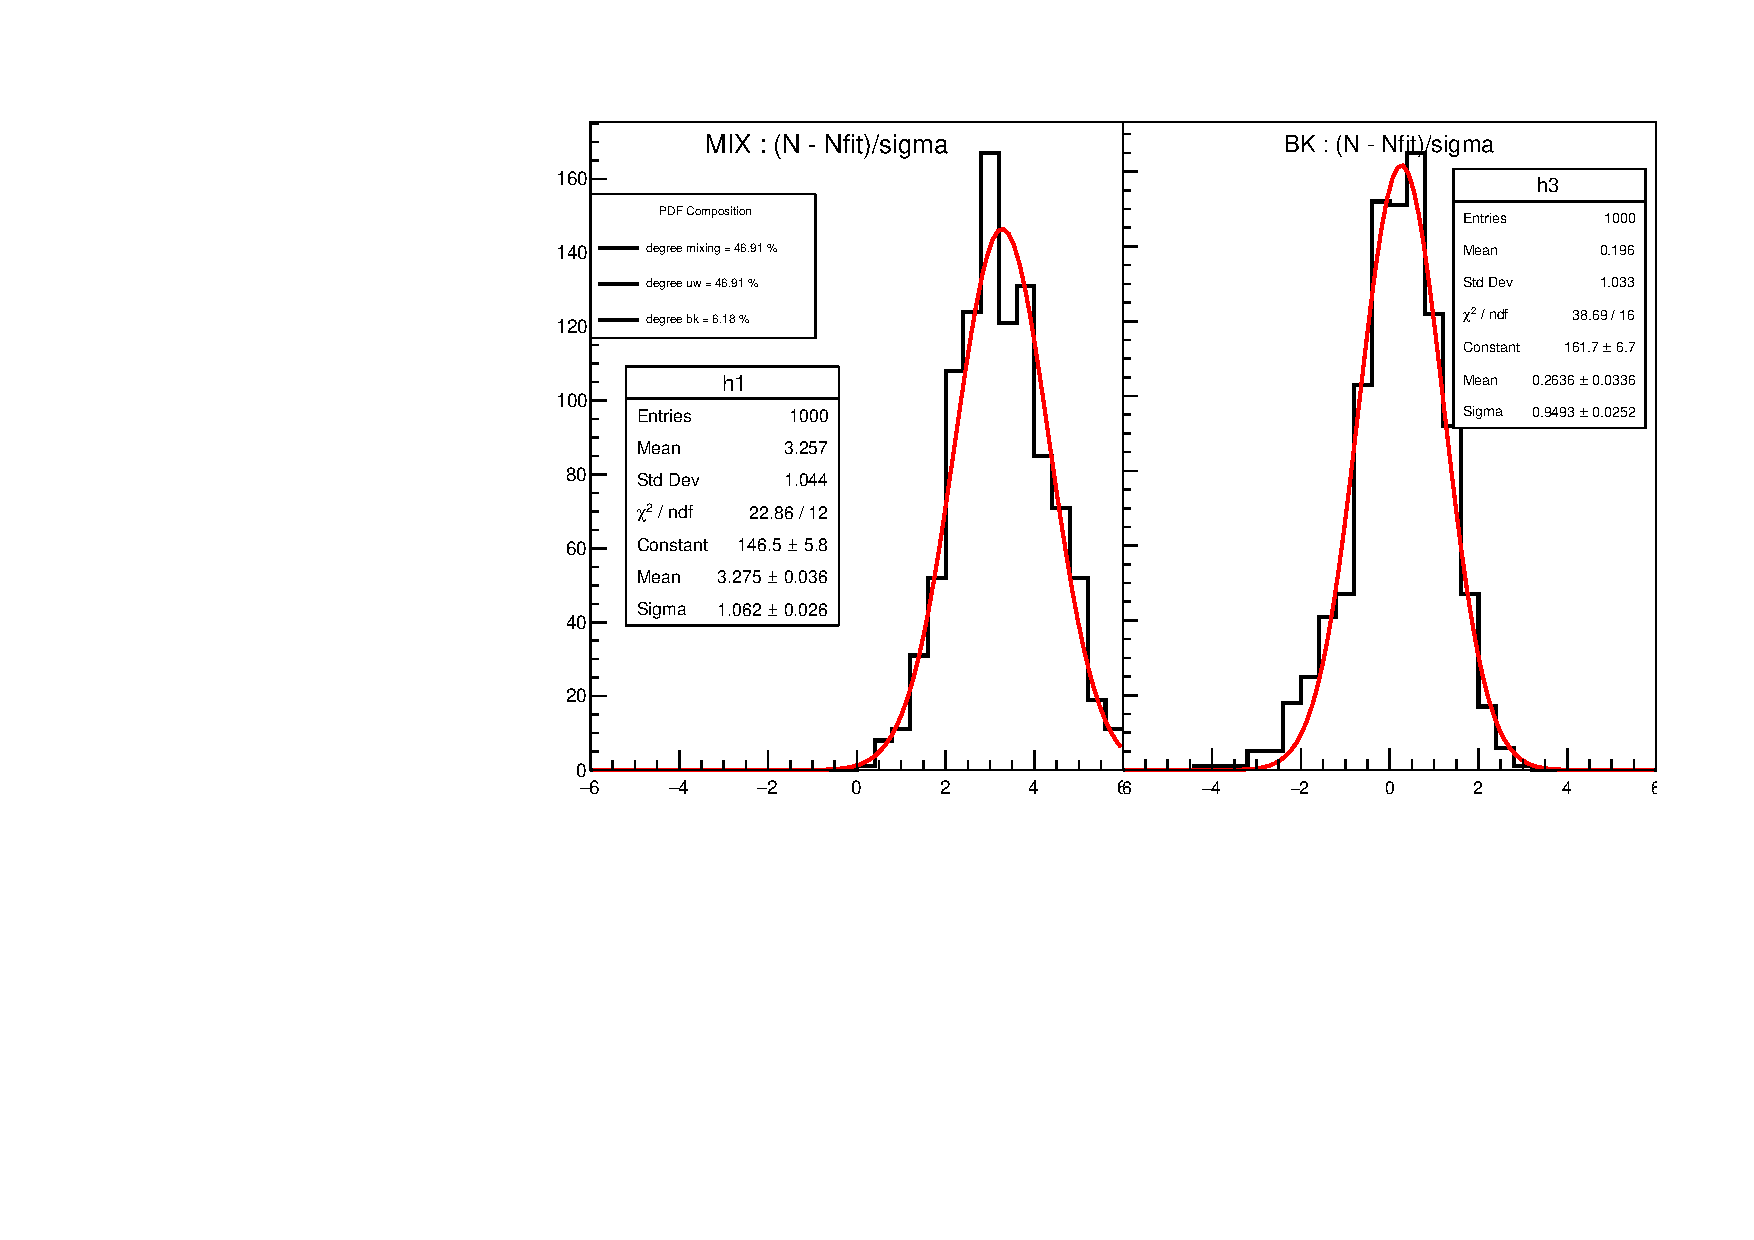
\includegraphics[width = 0.8\textwidth]{N165/ToyNmixNbk,NuwFixed(46,46,6).pdf}
\end{figure}
\end{frame}
}

{\nologo
\begin{frame}{$N_{uw}$ parameter of the fit model fixed}

We study the bias $N_{mix} - N_{reconstructed}$ with the parameter $N_{uw}$ of the fit model fixed to $0$. For small value of $w_{mix}$, corresponding to small contribution of \textit{Mixing}  (and, conversely, a significant contribution of \textit{Residual gas} PDF) we observe a large bias.

\begin{figure}
\subfloat{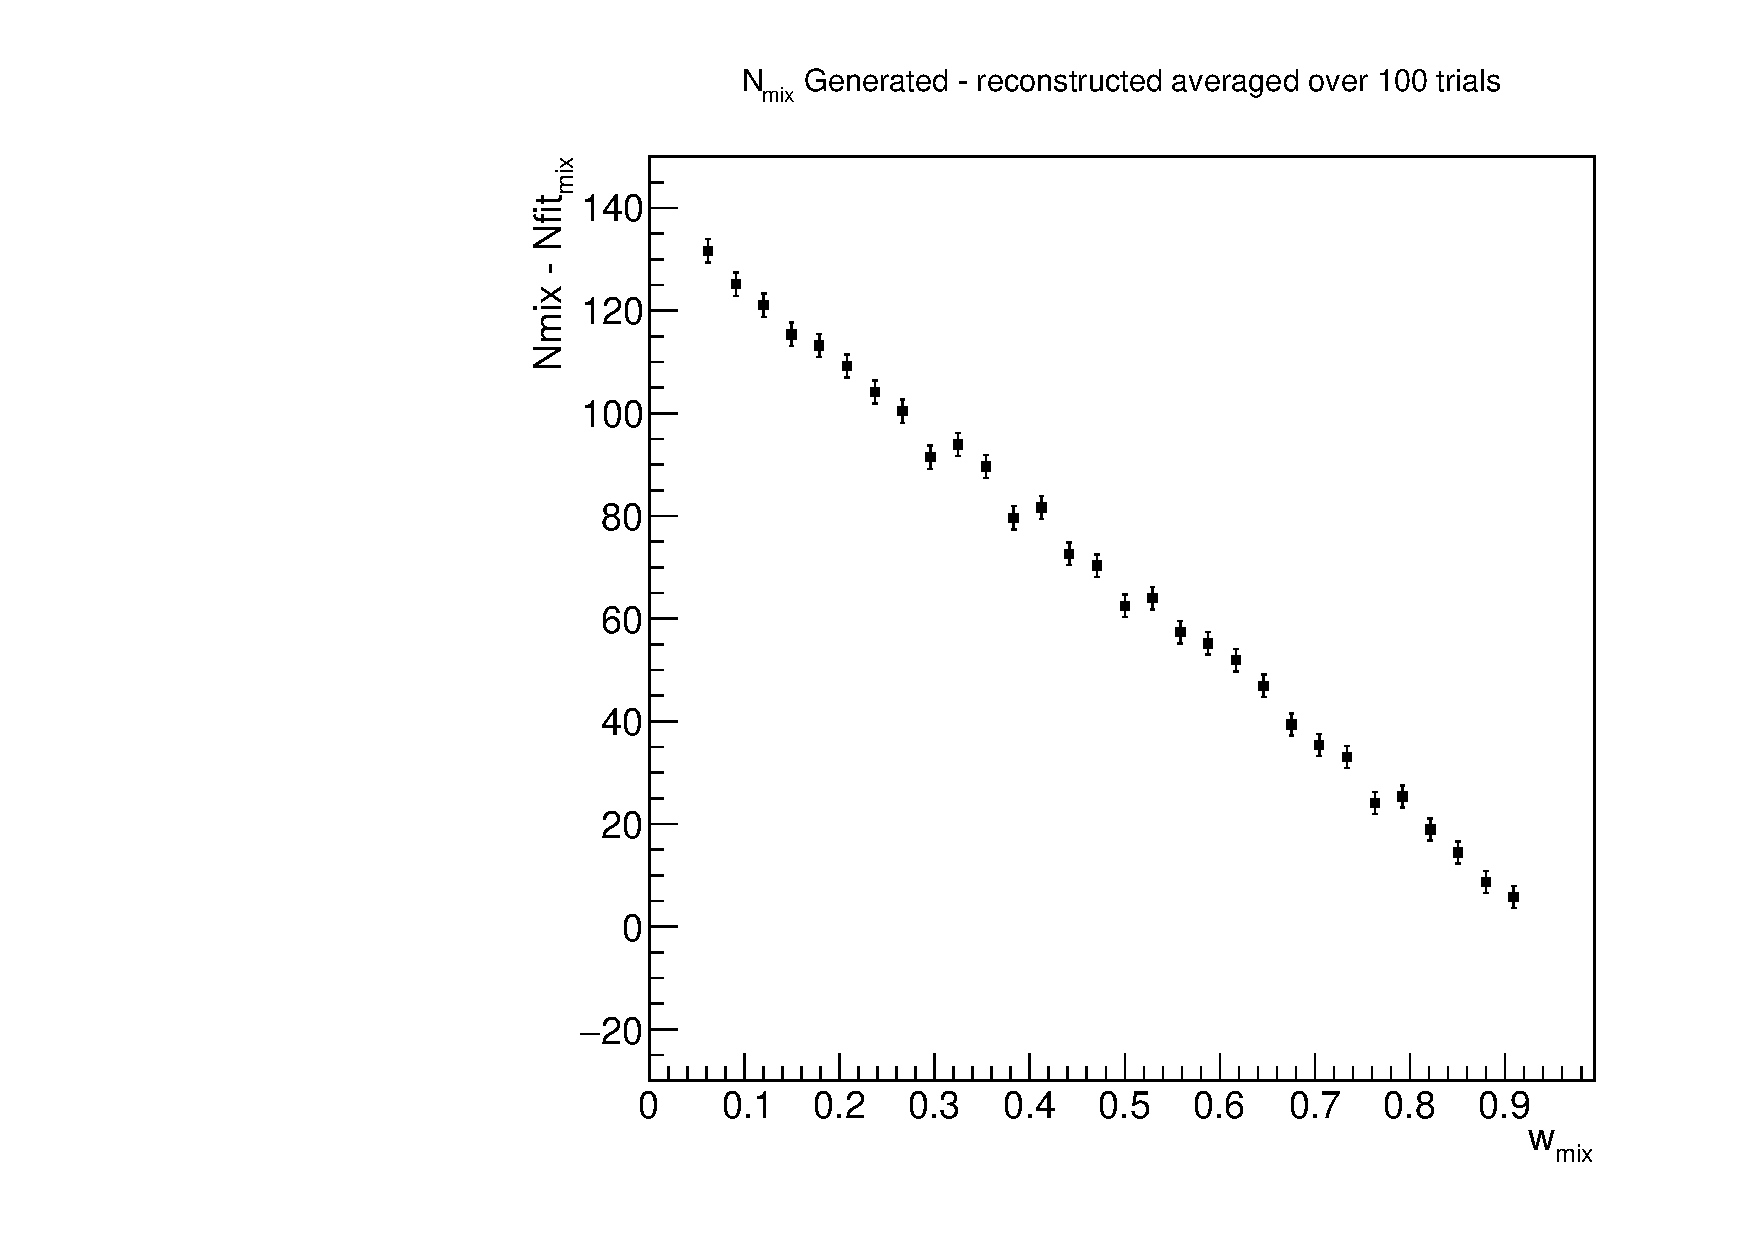
\includegraphics[width = 0.49\textwidth]{N165/Nmix,NuwFixed(84,9,6).pdf}}
\subfloat{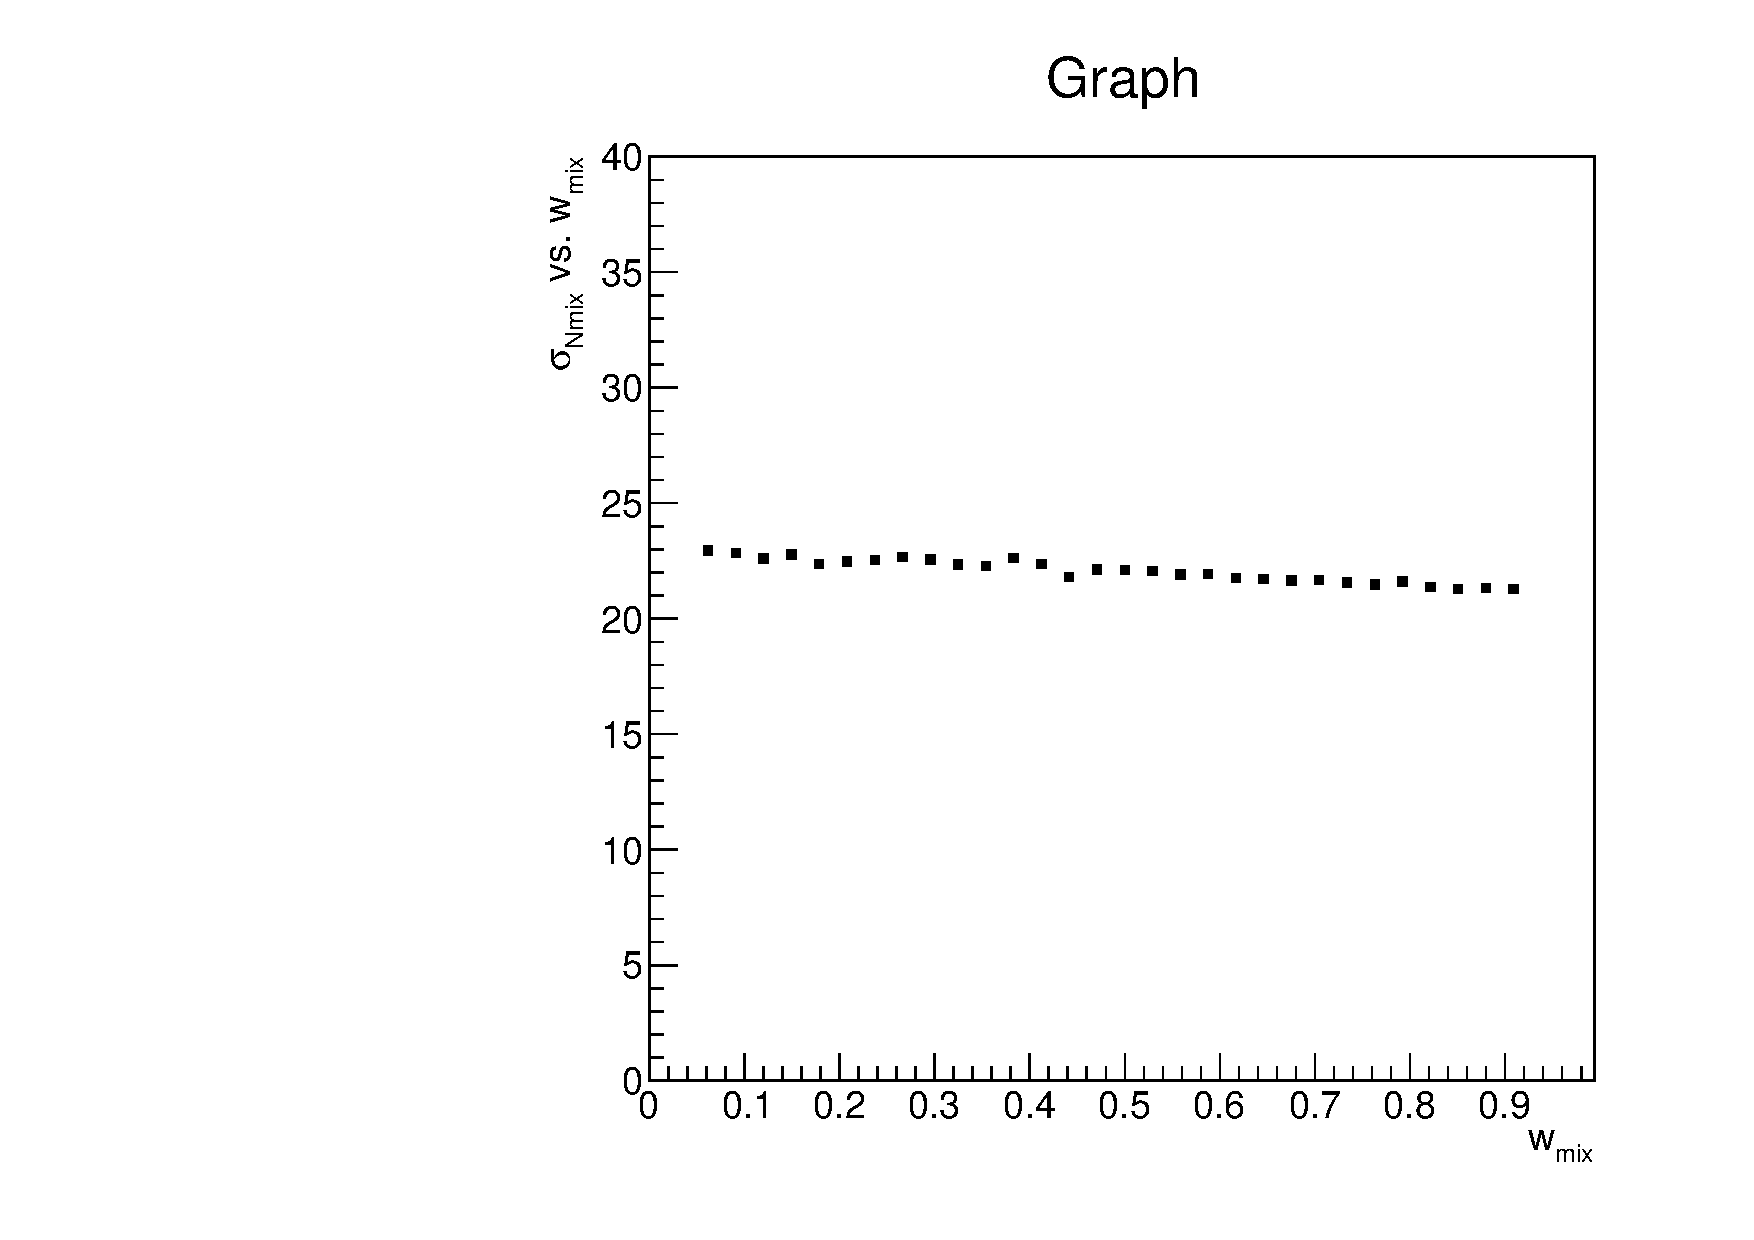
\includegraphics[width = 0.49\textwidth]{N165/sigmaNmix,NuwFixed(84,9,6).pdf}}
\end{figure}
\end{frame}
}
}
\end{document}